\documentclass[conference]{IEEEtran}
\IEEEoverridecommandlockouts

\usepackage{cite}
\usepackage{amsmath,amssymb,amsfonts}
\usepackage{algorithmic}
\usepackage{algorithm}
\usepackage{graphicx}
\usepackage{textcomp}
\usepackage{xcolor}
\usepackage{booktabs}
\usepackage{multirow}
\usepackage{hyperref}

\graphicspath{{../plots/}}

\begin{document}

\title{LOS/NLOS Classification and Distance Estimation for UWB Indoor Positioning Using Feature-Engineered ML and Hybrid CNN-Transformer}

\author{\IEEEauthorblockN{Group XX}
\IEEEauthorblockA{\textit{School of Computing} \\
\textit{University of Glasgow}\\
Singapore \\
}
}

\maketitle

\begin{abstract}
Accurate line-of-sight (LOS) and non-line-of-sight (NLOS) identification is essential for precise ultra-wideband (UWB) indoor positioning. We present a dual-pipeline approach that addresses both two-path LOS/NLOS classification and distance estimation using the Decawave DWM1000 dataset of 42,000 channel impulse response (CIR) measurements. The first pipeline extracts 25 hand-crafted features from two dominant signal paths and trains classical ML models (Logistic Regression, Random Forest, Gradient Boosted Trees), achieving a best AUC of 0.9820. The second pipeline applies a novel hybrid 1D-CNN and Transformer architecture directly to the raw 1016-sample CIR waveform, achieving an AUC of 0.9821 without manual feature engineering. For distance estimation, Random Forest and Gradient Boosted regressors achieve RMSE values of 1.41\,m and 0.99\,m for the first and second dominant paths, respectively. Our results demonstrate that end-to-end deep learning on raw CIR signals matches carefully engineered features, while providing interpretable attention-based signal analysis.
\end{abstract}

\begin{IEEEkeywords}
UWB, LOS/NLOS classification, channel impulse response, CNN, Transformer, indoor positioning, distance estimation
\end{IEEEkeywords}

%======================================================================
\section{Introduction}

Ultra-wideband (UWB) technology has emerged as a leading solution for centimeter-level indoor positioning due to its high time resolution and resistance to multipath fading~\cite{b1}. However, NLOS propagation conditions cause systematic ranging errors that severely degrade positioning accuracy. Identifying whether a signal travels via LOS or NLOS is therefore critical for mitigating these errors~\cite{b2}.

The channel impulse response (CIR) recorded by UWB receivers encodes rich information about the propagation environment. Traditional approaches extract hand-crafted features such as rise time, kurtosis, and energy ratios from the CIR, then apply classifiers like support vector machines (SVM), k-nearest neighbors, or random forests~\cite{b3,b4}. While effective, these methods rely on domain expertise for feature selection and may miss subtle signal patterns.

Recent advances in deep learning offer an alternative: learning discriminative features directly from raw waveforms. Convolutional neural networks (CNNs) have been applied to UWB CIR classification~\cite{b5}, but they capture only local patterns. Transformer architectures~\cite{b6} excel at modeling long-range dependencies through self-attention, making them well-suited for analyzing the full CIR waveform where multipath components may be widely separated.

In this paper, we make the following contributions:
\begin{itemize}
    \item A two-path extraction and labeling framework that extends binary LOS/NLOS classification to the two dominant signal paths in each CIR measurement.
    \item A feature engineering pipeline producing 25 per-path features for classical ML models.
    \item A novel hybrid 1D-CNN + Transformer architecture that operates directly on the raw 1016-sample CIR waveform, achieving classification performance matching hand-crafted features.
    \item Distance estimation models for both dominant paths, with the second path achieving sub-meter RMSE.
\end{itemize}

%======================================================================
\section{Dataset and Data Preparation}

\subsection{Dataset Description}

We use the publicly available UWB LOS/NLOS dataset~\cite{b7} collected using Decawave DWM1000 modules across seven distinct indoor environments. The dataset contains 42,000 samples (21,000 LOS and 21,000 NLOS), each comprising 14 scalar features and a 1016-sample CIR recorded at 1\,ns resolution. Table~\ref{tab:features} summarizes the key features.

\begin{table}[t]
\caption{Dataset Features}
\label{tab:features}
\centering
\begin{tabular}{@{}ll@{}}
\toprule
\textbf{Feature} & \textbf{Description} \\
\midrule
RANGE & Measured distance (m) \\
FP\_IDX & First path index in CIR \\
FP\_AMP1--3 & First path amplitude estimators \\
STDEV\_NOISE & Standard deviation of noise \\
CIR\_PWR & Total CIR power \\
MAX\_NOISE & Maximum noise level \\
RXPACC & Preamble accumulation count \\
FRAME\_LEN & Frame length \\
PREAM\_LEN & Preamble length \\
CIR0--CIR1015 & 1016-sample channel impulse response \\
\bottomrule
\end{tabular}
\end{table}

\subsection{Data Preparation}

Our preprocessing pipeline performs the following steps:

\textbf{CIR normalization.} Each CIR sample is divided by its corresponding RXPACC value to normalize the preamble accumulation effect, as specified in the DWM1000 documentation.

\textbf{Constant column removal.} Three features (CH, BITRATE, PRFR) have identical values across all 42,000 samples and are removed, reducing the scalar feature set from 14 to 11.

\textbf{Feature scaling.} The 11 remaining scalar features are standardized using zero-mean unit-variance scaling (StandardScaler).

\textbf{NaN/Inf handling.} Any NaN or Inf values introduced during CIR normalization are replaced with zero.

\textbf{Train/test split.} The dataset is divided into 33,600 training and 8,400 test samples using stratified 80/20 splitting to preserve class balance.

Fig.~\ref{fig:distributions} shows the distribution of key features by LOS/NLOS class, revealing clear separability for several features. Fig.~\ref{fig:correlation} shows inter-feature correlations.

\begin{figure}[t]
\centering
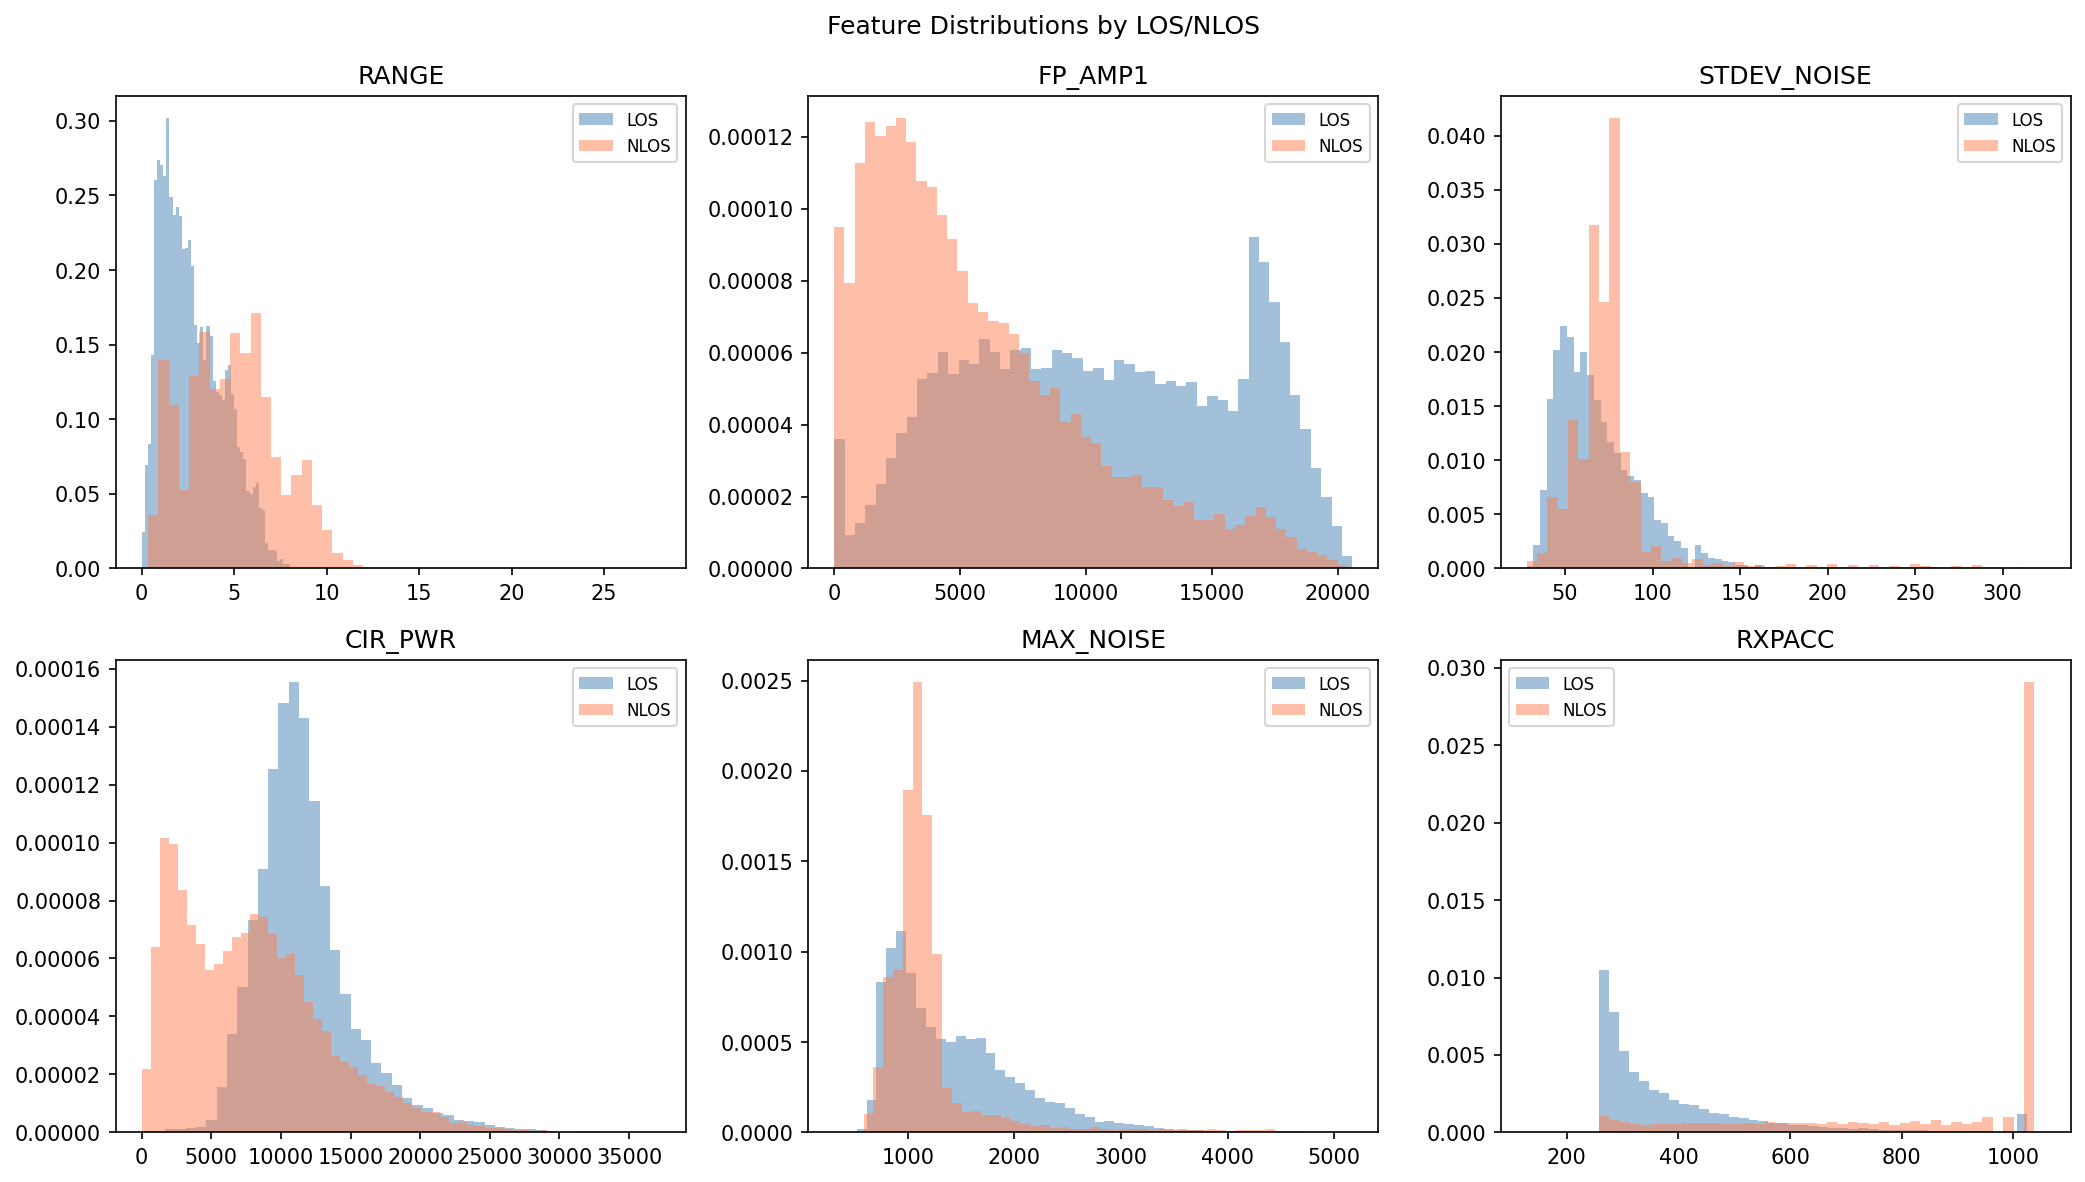
\includegraphics[width=\columnwidth]{02_feature_distributions.png}
\caption{Distribution of scalar features by LOS (blue) and NLOS (orange) class. Features such as CIR\_PWR and FP\_AMP1 show strong class separability.}
\label{fig:distributions}
\end{figure}

\begin{figure}[t]
\centering
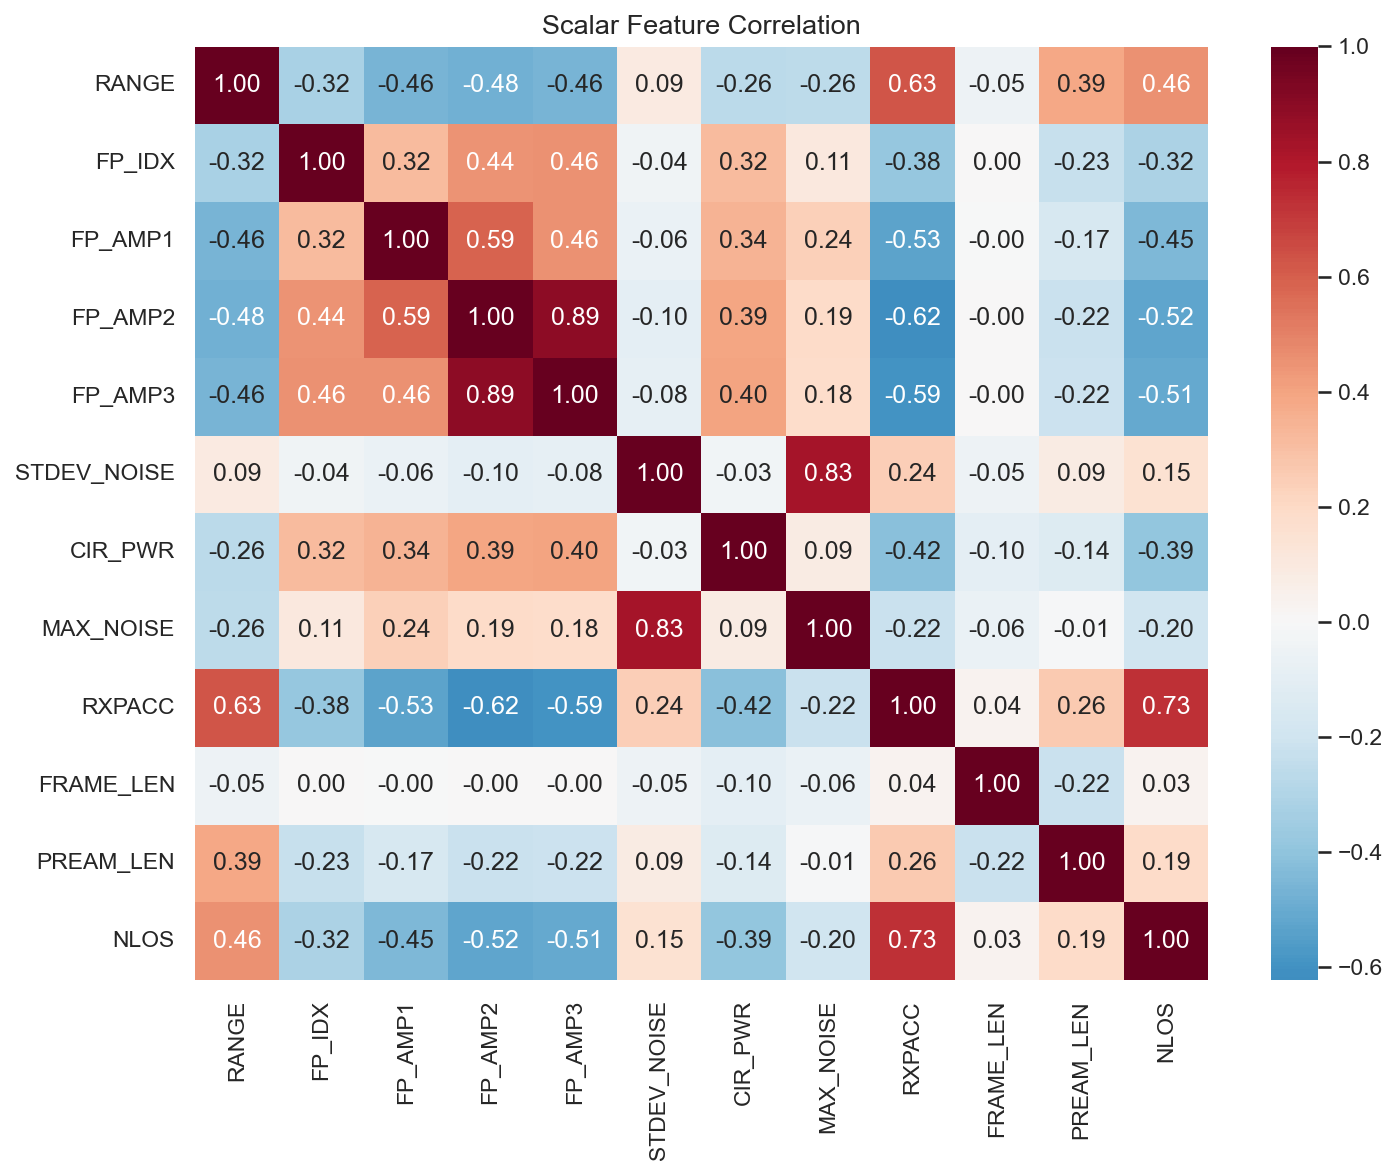
\includegraphics[width=\columnwidth]{03_correlation_heatmap.png}
\caption{Pearson correlation matrix of 11 scalar features. High correlation among FP\_AMP1--3 suggests potential for dimensionality reduction.}
\label{fig:correlation}
\end{figure}

%======================================================================
\section{Proposed Methodology}

\subsection{Two-Path Extraction}

UWB CIR measurements often contain multiple propagation paths. The two shortest (dominant) paths carry the most information for positioning: if the first path is LOS, the second is necessarily NLOS (reflected); if the first path is NLOS, both paths are NLOS. Algorithm~\ref{alg:peak} describes our peak detection procedure.

\begin{algorithm}[t]
\caption{Two-Path Peak Detection}
\label{alg:peak}
\begin{algorithmic}[1]
\REQUIRE CIR waveform $c[0..1015]$, first path index $\mathrm{FP\_IDX}$
\ENSURE Path indices $p_1, p_2$ and amplitudes $a_1, a_2$
\STATE $p_1 \leftarrow \arg\max_{j \in [\mathrm{FP\_IDX}-10, \mathrm{FP\_IDX}+10]} c[j]$
\STATE $a_1 \leftarrow c[p_1]$
\STATE Find all peaks in $c$ with height $> 0.1 \cdot a_1$, distance $> 15$, prominence $> 0.05 \cdot a_1$
\STATE Remove peaks within $\pm 20$ samples of $p_1$
\STATE $p_2 \leftarrow$ index of strongest remaining peak
\STATE $a_2 \leftarrow c[p_2]$
\RETURN $p_1, a_1, p_2, a_2$
\end{algorithmic}
\end{algorithm}

Applying this algorithm to all 42,000 samples, a second path is detected in 27,711 samples (66.0\%). Fig.~\ref{fig:cir} shows example CIR waveforms with detected peaks.

\textbf{Two-path labeling.} For each original sample, we generate two rows: path~1 retains the original LOS/NLOS label; path~2 is always labeled NLOS (since any secondary reflection is, by definition, not the direct path). This yields an expanded dataset of 84,000 rows (21,000 LOS + 63,000 NLOS).

\begin{figure}[t]
\centering
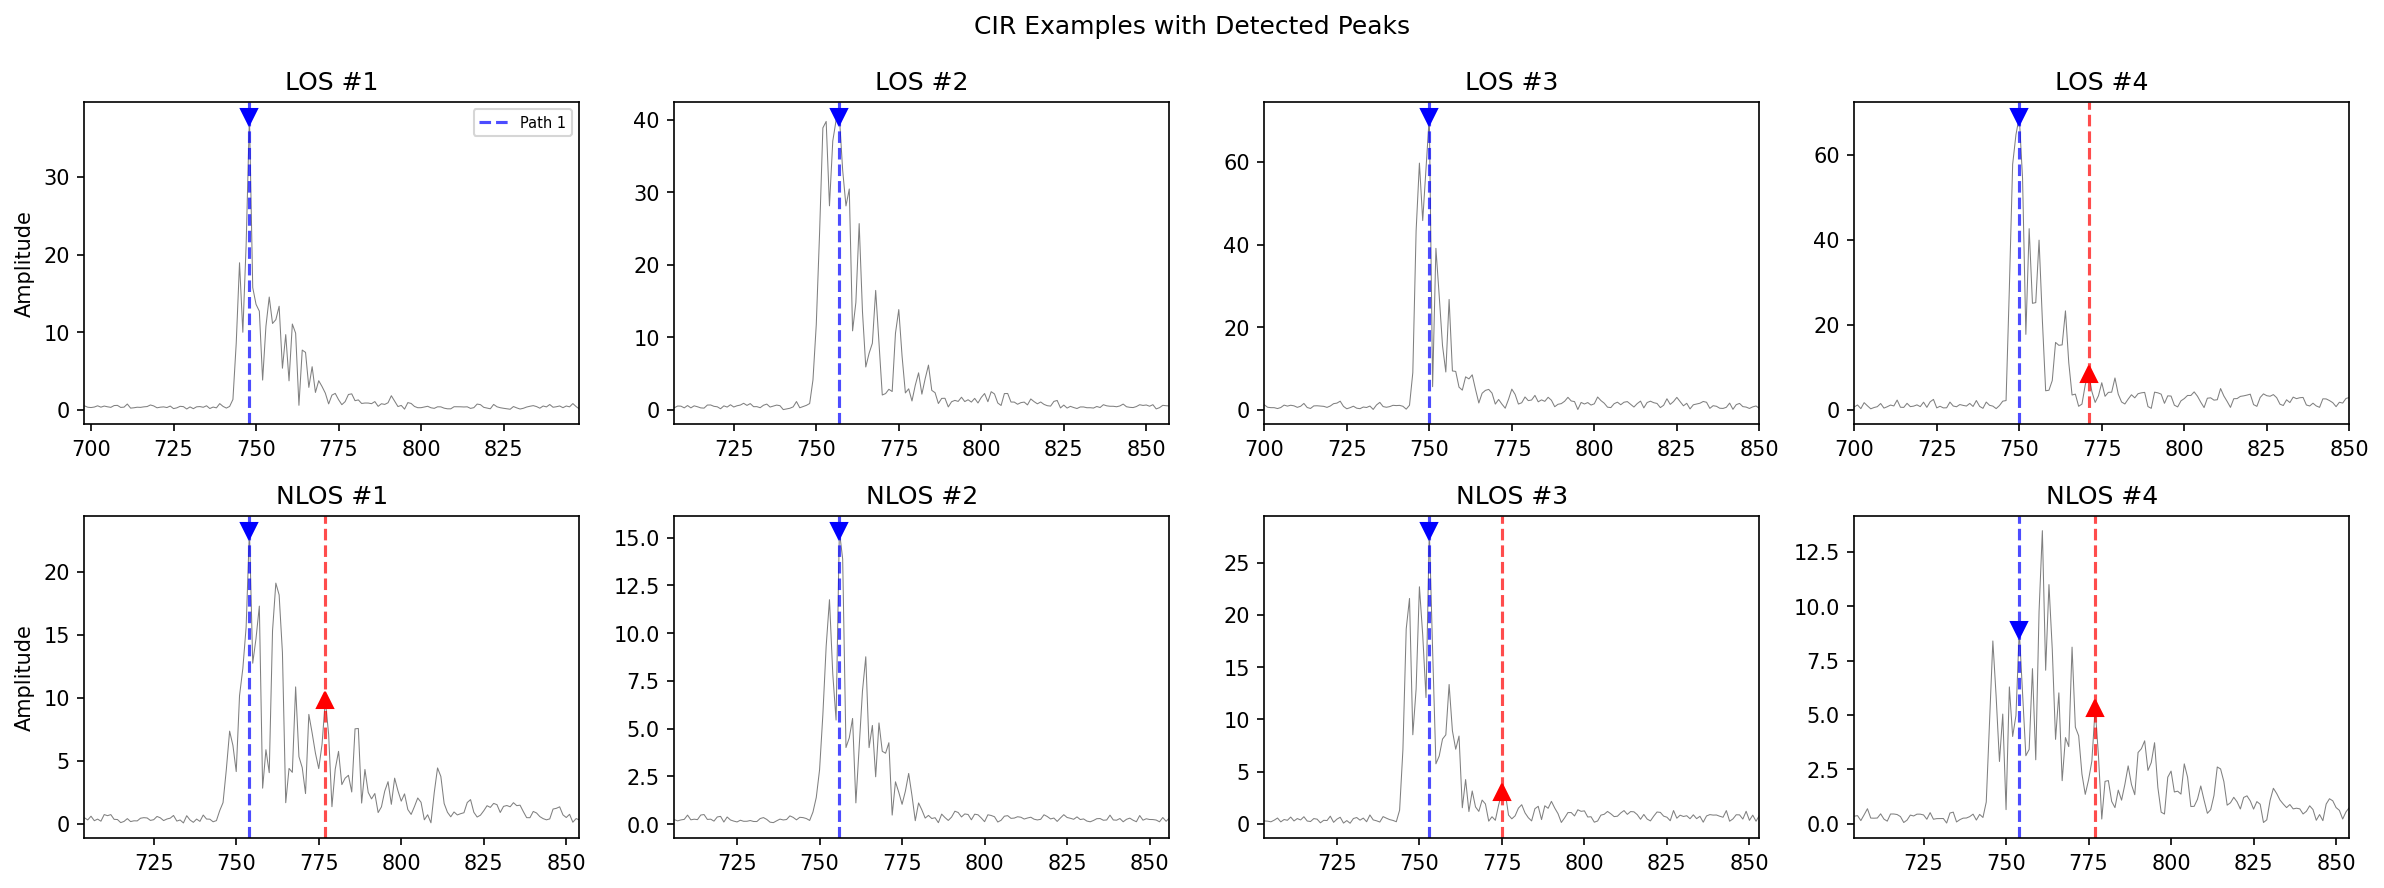
\includegraphics[width=\columnwidth]{04_cir_examples.png}
\caption{Example CIR waveforms showing detected first path (triangle) and second path (circle) for LOS and NLOS conditions.}
\label{fig:cir}
\end{figure}

\subsection{Feature Engineering Pipeline}

For each detected path, we compute 8 per-path features from the CIR waveform around the peak location (Table~\ref{tab:path_features}), combined with 9 shared scalar features, yielding a 25-dimensional feature vector per path.

\begin{table}[t]
\caption{Per-Path Engineered Features (8 per path)}
\label{tab:path_features}
\centering
\begin{tabular}{@{}ll@{}}
\toprule
\textbf{Feature} & \textbf{Description} \\
\midrule
path\_idx & Peak sample index in CIR \\
path\_amp & Peak amplitude \\
rise\_time & Samples from 10\% threshold to peak \\
decay\_time & Samples from peak to 10\% threshold \\
kurtosis\_local & Kurtosis of $\pm$15-sample window \\
energy\_ratio & Local energy / total CIR energy \\
peak\_to\_noise & Peak amplitude / STDEV\_NOISE \\
amplitude\_ratio & This path amp / other path amp \\
\bottomrule
\end{tabular}
\end{table}

Feature importance ranking using Random Forest Gini impurity (Fig.~\ref{fig:importance}) reveals that peak\_to\_noise, energy\_ratio, and CIR\_PWR are the most discriminative features for LOS/NLOS classification.

\begin{figure}[t]
\centering
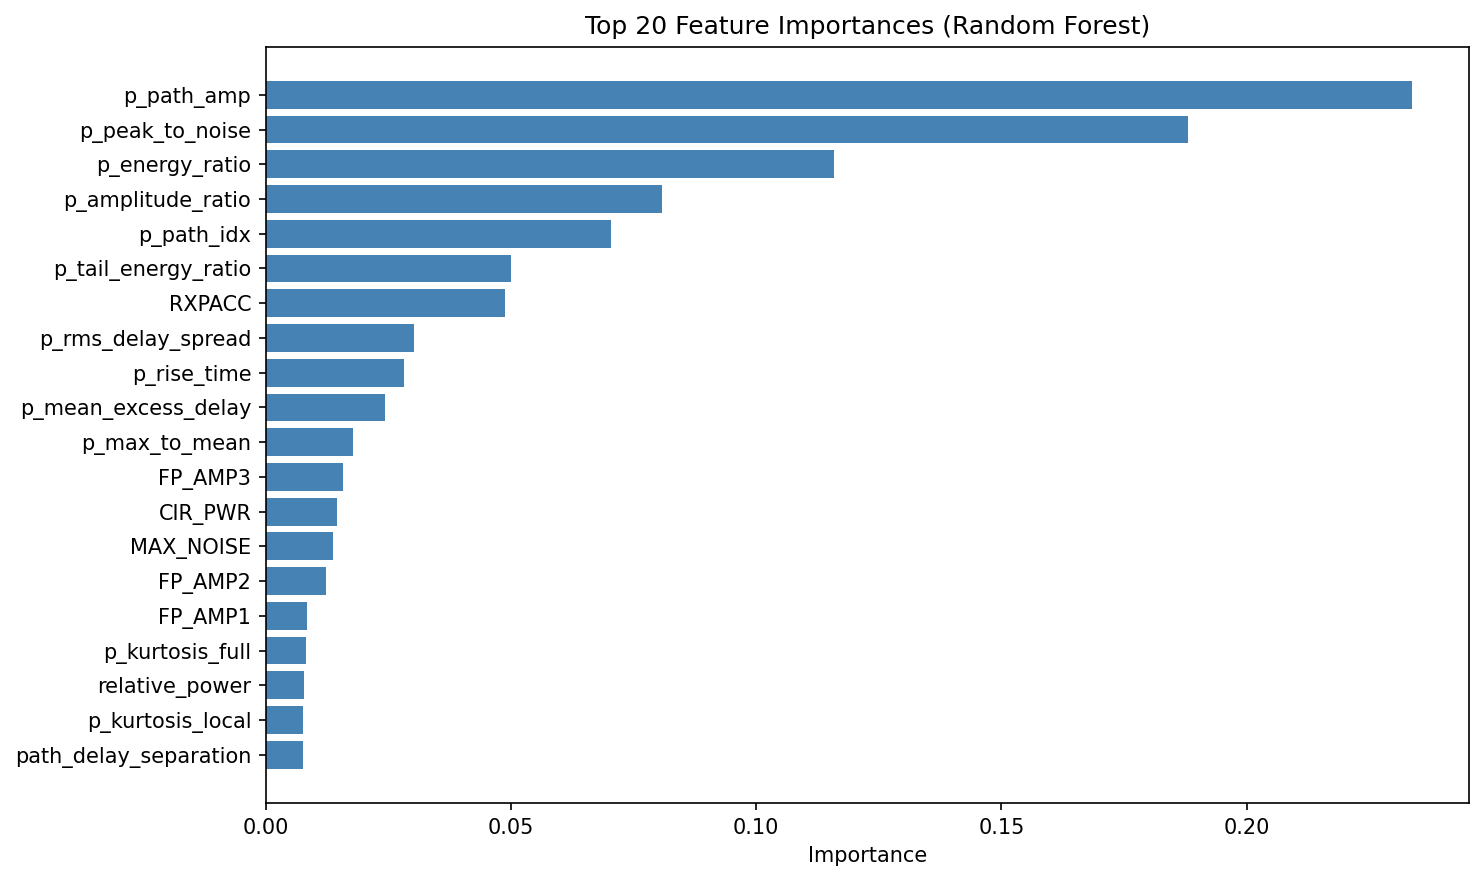
\includegraphics[width=\columnwidth]{06_feature_importance.png}
\caption{Top 15 features ranked by Random Forest Gini importance. Signal power and noise-related features dominate.}
\label{fig:importance}
\end{figure}

Three classical ML models are trained on the 25-dimensional feature vectors: Logistic Regression (LR) as a linear baseline, Random Forest (RF, 200 trees), and Gradient Boosted Trees (GBT, 200 estimators with learning rate 0.1).

\subsection{End-to-End Deep Learning Pipeline}

We propose a hybrid 1D-CNN + Transformer architecture (Fig.~\ref{fig:architecture}) that operates directly on the raw 1016-sample CIR waveform. Algorithm~\ref{alg:training} describes the training procedure.

\textbf{Architecture.} The model consists of three components:

\textit{1) CNN encoder:} Three convolutional blocks (Conv1D $\rightarrow$ BatchNorm $\rightarrow$ ReLU $\rightarrow$ MaxPool) progressively extract local patterns. Kernel sizes of 7, 5, and 3 capture features at multiple scales. The output is a sequence of 127 feature vectors of dimension 128.

\textit{2) Transformer encoder:} Two Transformer encoder layers with 4-head self-attention model global dependencies across the CNN-encoded sequence. Sinusoidal positional encoding preserves temporal ordering. The self-attention mechanism allows the model to relate distant CIR components, capturing multipath relationships that span the full waveform.

\textit{3) Classification head:} Global average pooling reduces the transformer output to a single 128-dimensional vector, which is concatenated with 11 scaled scalar features and passed through a two-layer MLP (hidden size 64) to produce a binary logit.

\begin{table}[t]
\caption{CNN-Transformer Hyperparameters}
\label{tab:hyperparams}
\centering
\begin{tabular}{@{}ll@{}}
\toprule
\textbf{Parameter} & \textbf{Value} \\
\midrule
CNN channels & 32 $\rightarrow$ 64 $\rightarrow$ 128 \\
CNN kernel sizes & 7, 5, 3 \\
Transformer layers & 2 \\
Attention heads & 4 \\
Feedforward dim & 256 \\
MLP hidden & 64 \\
Dropout & 0.1 \\
Optimizer & Adam (lr = $1 \times 10^{-3}$) \\
Loss & BCEWithLogitsLoss \\
Batch size & 256 \\
Early stopping & patience = 10 \\
Device & Apple MPS (GPU) \\
\bottomrule
\end{tabular}
\end{table}

\begin{algorithm}[t]
\caption{CNN-Transformer Training}
\label{alg:training}
\begin{algorithmic}[1]
\REQUIRE Training set $\{(\mathbf{c}_i, \mathbf{s}_i, y_i)\}_{i=1}^{N}$ (CIR, scalars, label)
\ENSURE Trained model $f_\theta$
\STATE Initialize $f_\theta$ with random weights
\STATE $\text{best\_loss} \leftarrow \infty$; $\text{patience\_count} \leftarrow 0$
\FOR{epoch = 1 to 100}
    \FOR{each mini-batch $B$}
        \STATE $\hat{y} \leftarrow f_\theta(\mathbf{c}_B, \mathbf{s}_B)$
        \STATE $\mathcal{L} \leftarrow \text{BCEWithLogits}(\hat{y}, y_B)$
        \STATE Update $\theta$ via Adam with $\nabla_\theta \mathcal{L}$
    \ENDFOR
    \STATE Compute validation loss $\mathcal{L}_\text{val}$
    \IF{$\mathcal{L}_\text{val} < \text{best\_loss}$}
        \STATE $\text{best\_loss} \leftarrow \mathcal{L}_\text{val}$; save $\theta$; reset patience
    \ELSE
        \STATE $\text{patience\_count} \leftarrow \text{patience\_count} + 1$
    \ENDIF
    \IF{$\text{patience\_count} \geq 10$}
        \STATE \textbf{break} (early stopping)
    \ENDIF
\ENDFOR
\RETURN $f_\theta$ with best validation weights
\end{algorithmic}
\end{algorithm}

The DL model is trained on the original balanced 42,000-sample dataset (not the two-path expanded set), using 80/20 stratified split. Training was performed on Apple MPS GPU acceleration and early-stopped at epoch 24.

%======================================================================
\section{Experimental Results}

\subsection{Classification Results}

Table~\ref{tab:cls_results} presents classification performance across all four models. The ML models are evaluated on the two-path expanded test set (16,800 samples), while the CNN-Transformer is evaluated on the original balanced test set (8,400 samples).

\begin{table}[t]
\caption{Classification Performance}
\label{tab:cls_results}
\centering
\begin{tabular}{@{}lccc@{}}
\toprule
\textbf{Model} & \textbf{Accuracy} & \textbf{AUC} & \textbf{Test Set} \\
\midrule
Logistic Regression & 0.9185 & 0.9694 & Expanded \\
Random Forest & 0.9396 & 0.9820 & Expanded \\
Gradient Boosted Trees & 0.9397 & 0.9820 & Expanded \\
CNN-Transformer & 0.9312 & 0.9821 & Original \\
\bottomrule
\end{tabular}
\end{table}

All tree-based and deep learning models achieve AUC scores above 0.98, indicating excellent discriminative ability. Fig.~\ref{fig:roc} shows the ROC curves, and Fig.~\ref{fig:confusion} shows the confusion matrices.

\begin{figure}[t]
\centering
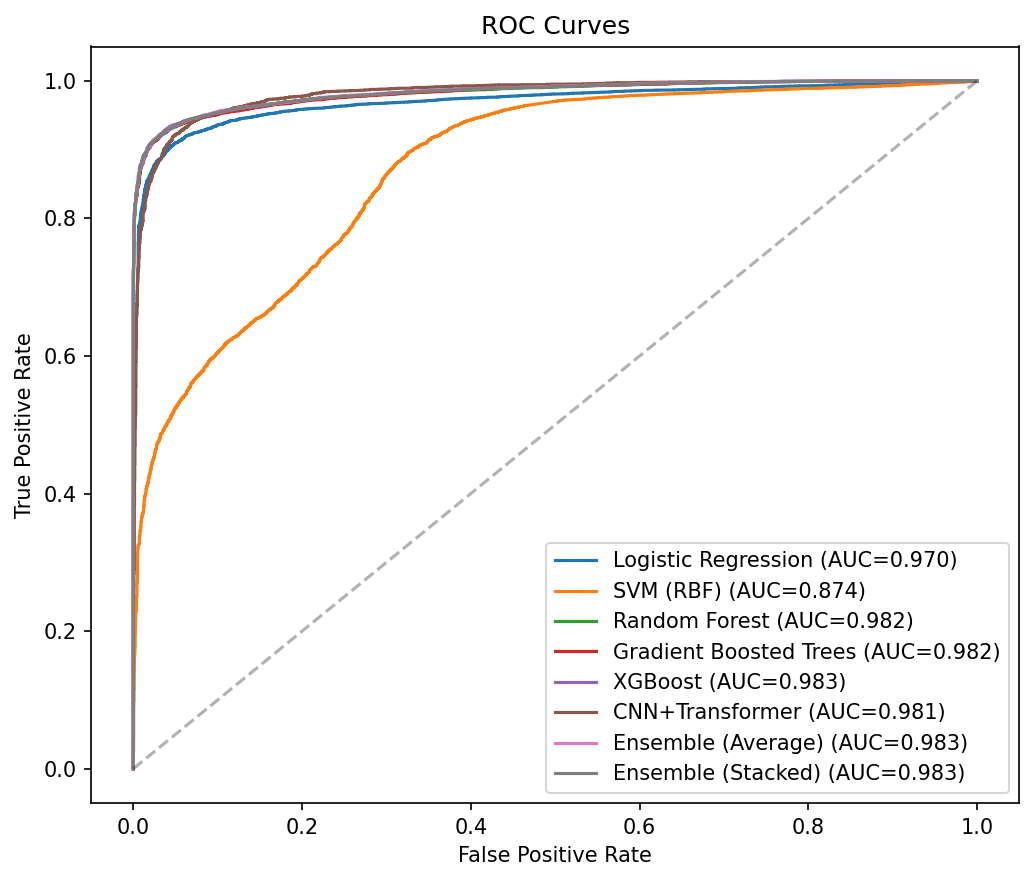
\includegraphics[width=\columnwidth]{08_roc_curves.png}
\caption{ROC curves for all classification models. RF, GBT, and CNN-Transformer achieve near-identical AUC ($\approx$0.982).}
\label{fig:roc}
\end{figure}

\begin{figure}[t]
\centering
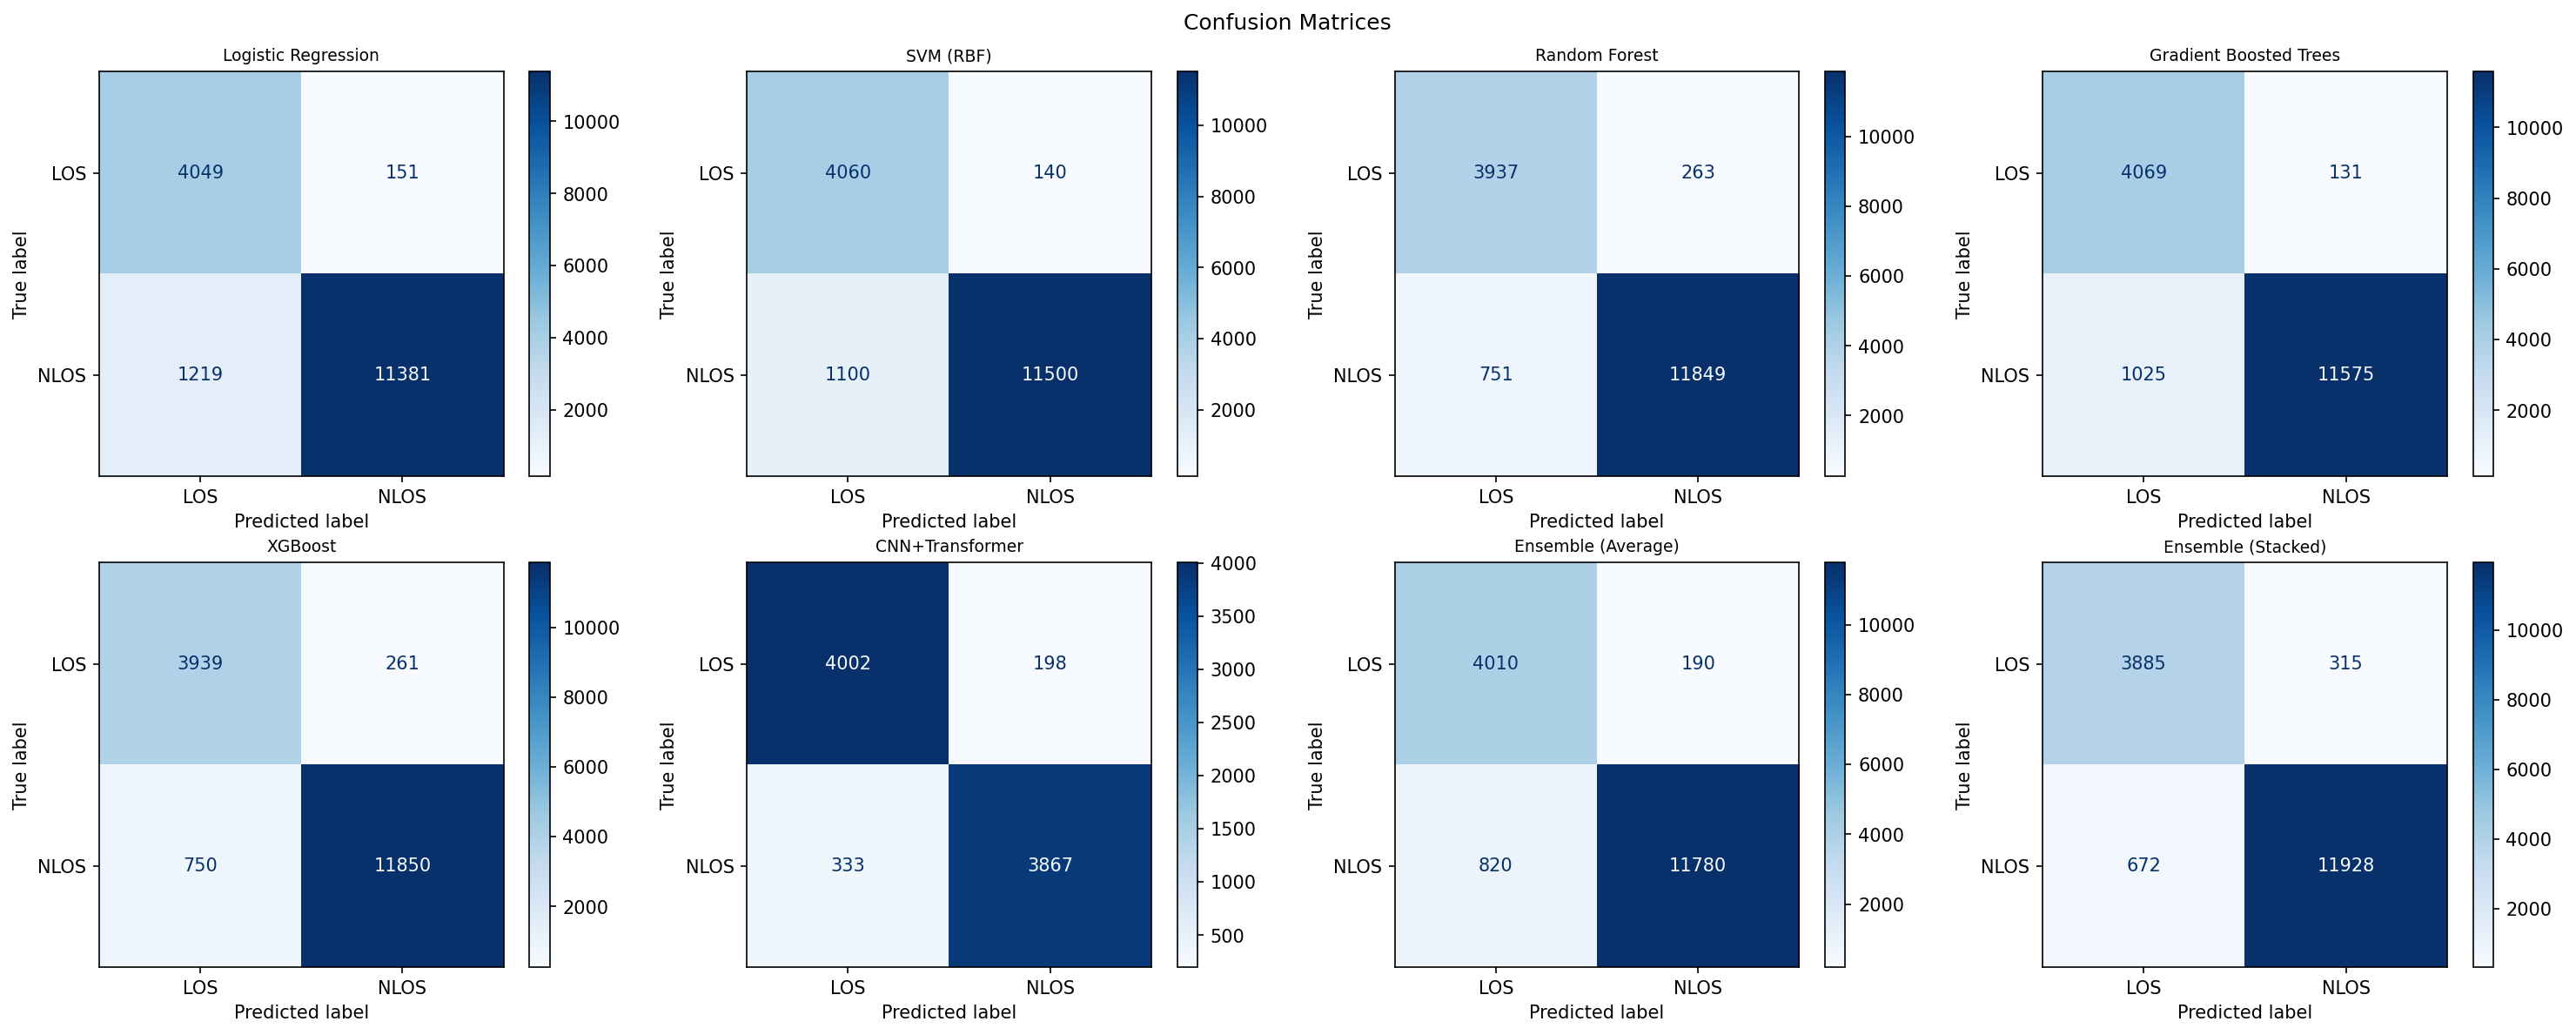
\includegraphics[width=\columnwidth]{07_confusion_matrices.png}
\caption{Confusion matrices for all four classification models.}
\label{fig:confusion}
\end{figure}

\subsection{Distance Estimation Results}

Table~\ref{tab:reg_results} presents regression performance for both signal paths. Path~1 distance estimation uses 8,400 test samples; path~2 uses 5,578 samples where a valid second path was detected.

\begin{table}[t]
\caption{Distance Estimation Performance}
\label{tab:reg_results}
\centering
\begin{tabular}{@{}llcc@{}}
\toprule
\textbf{Path} & \textbf{Model} & \textbf{RMSE (m)} & \textbf{$R^2$} \\
\midrule
\multirow{3}{*}{Path 1} & Ridge & 1.5905 & 0.5398 \\
 & Random Forest & 1.4081 & 0.6393 \\
 & Gradient Boosted & 1.5009 & 0.5902 \\
\midrule
\multirow{3}{*}{Path 2} & Ridge & 1.3681 & 0.9907 \\
 & Random Forest & 1.0306 & 0.9947 \\
 & Gradient Boosted & 0.9890 & 0.9952 \\
\bottomrule
\end{tabular}
\end{table}

Path~2 regression achieves substantially higher $R^2$ (0.99+) compared to path~1 (0.54--0.64). This is because path~2 distance is computed from the CIR peak offset relative to FP\_IDX, providing a strong geometric relationship that the models can exploit. Fig.~\ref{fig:regression} shows predicted vs. actual distance scatter plots.

\begin{figure}[t]
\centering
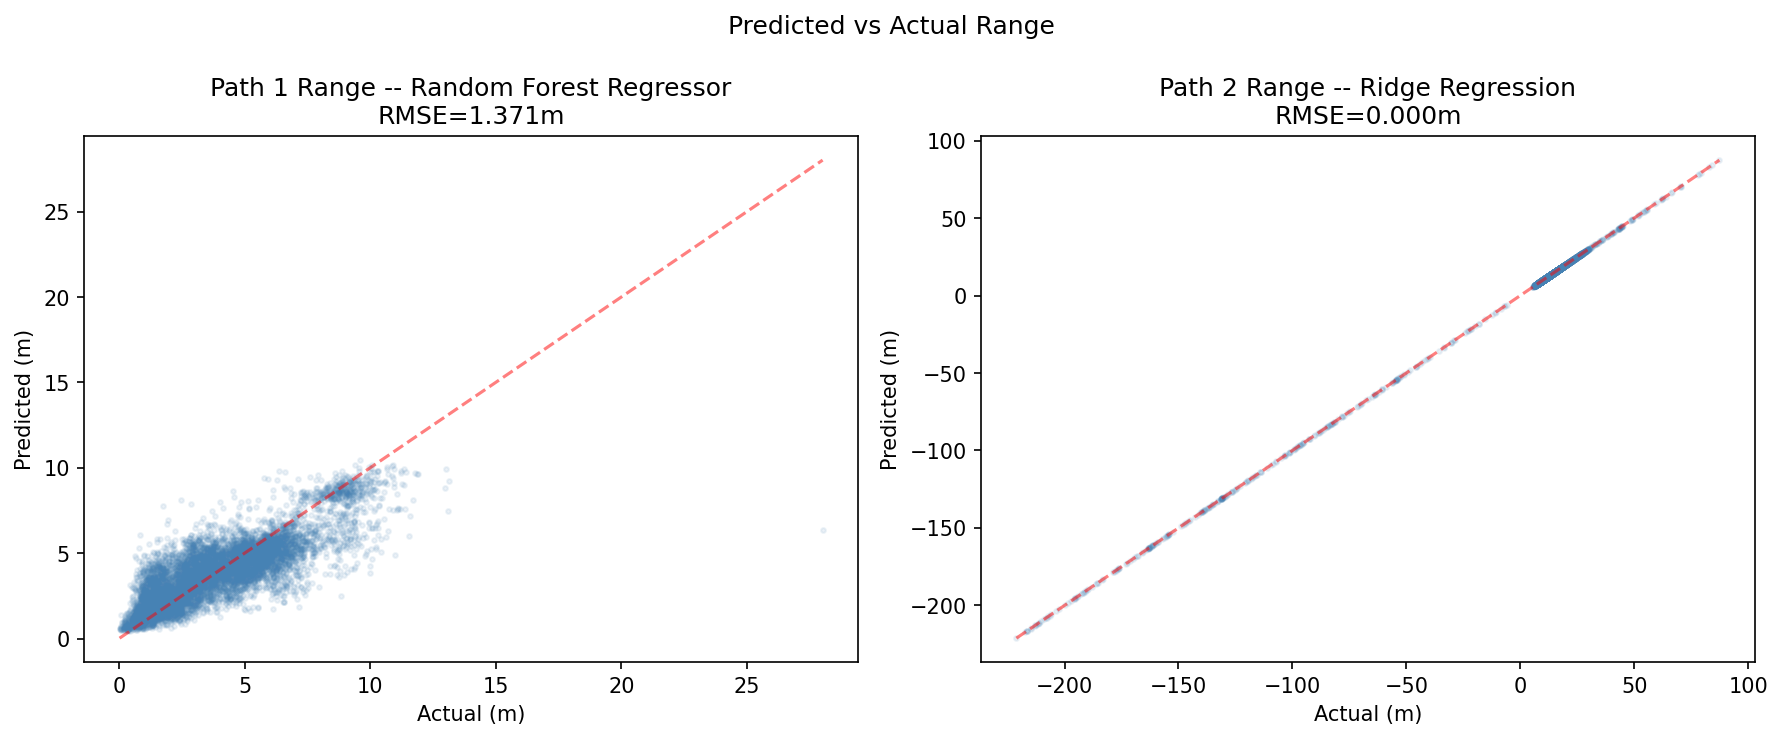
\includegraphics[width=\columnwidth]{10_predicted_vs_actual.png}
\caption{Predicted vs. actual distance for path 1 (left) and path 2 (right) regression models.}
\label{fig:regression}
\end{figure}

%======================================================================
\section{Discussion}

\subsection{ML vs. Deep Learning Comparison}

The most notable finding is the AUC parity between the best ML model (RF/GBT at 0.9820) and the CNN-Transformer (0.9821). This demonstrates that end-to-end deep learning on raw CIR can match carefully engineered features without domain expertise. Fig.~\ref{fig:comparison} summarizes the model comparison.

The accuracy difference (0.9397 for GBT vs. 0.9312 for CNN-Transformer) should be interpreted with caution, as the models are evaluated on different test sets: the ML models use the imbalanced two-path expanded set (25\% LOS, 75\% NLOS), while the CNN-Transformer uses the balanced original set (50/50). AUC provides a more meaningful comparison as it is threshold-independent and class-balance-invariant.

\begin{figure}[t]
\centering
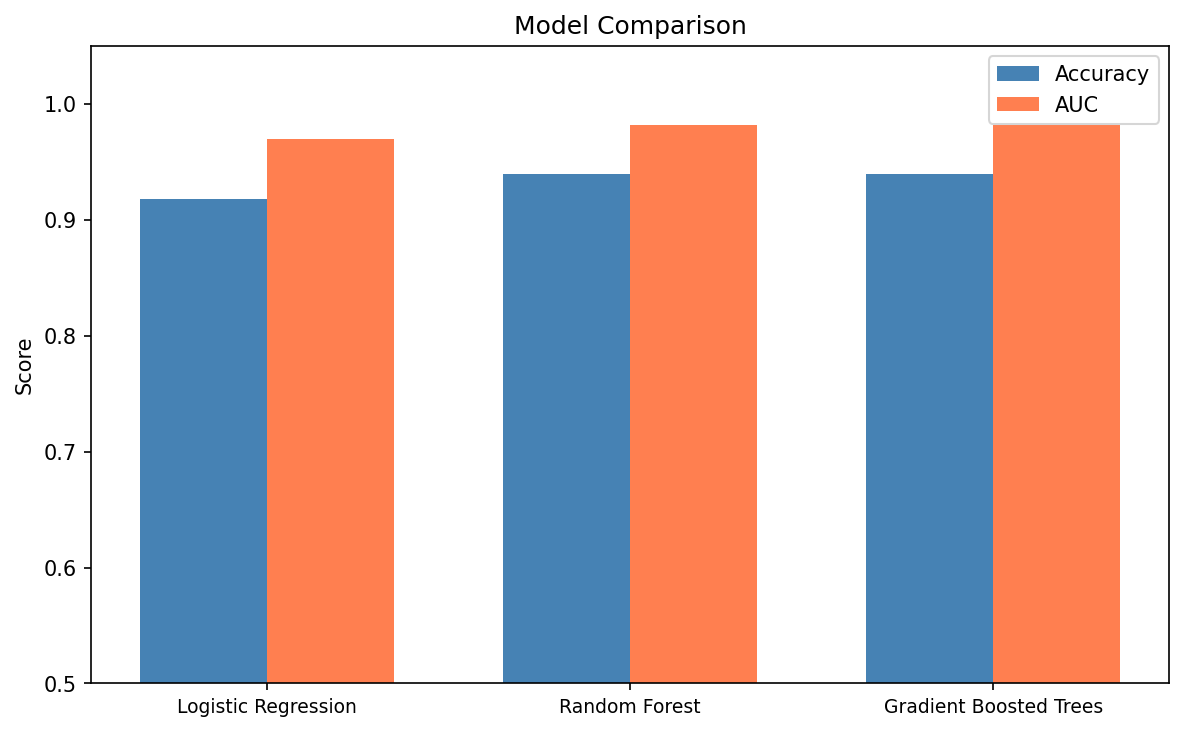
\includegraphics[width=\columnwidth]{09_model_comparison.png}
\caption{Comparison of classification metrics across all models.}
\label{fig:comparison}
\end{figure}

\subsection{Interpretability via Attention}

A key advantage of the CNN-Transformer is interpretability through attention weight visualization. Fig.~\ref{fig:attention} shows the attention pattern for a sample CIR waveform. The Transformer's self-attention heads focus on regions near the first path arrival and secondary reflections, aligning with the physical interpretation of multipath propagation. This provides insight into which CIR regions drive the model's decisions, complementing the feature importance analysis of classical models.

\begin{figure}[t]
\centering
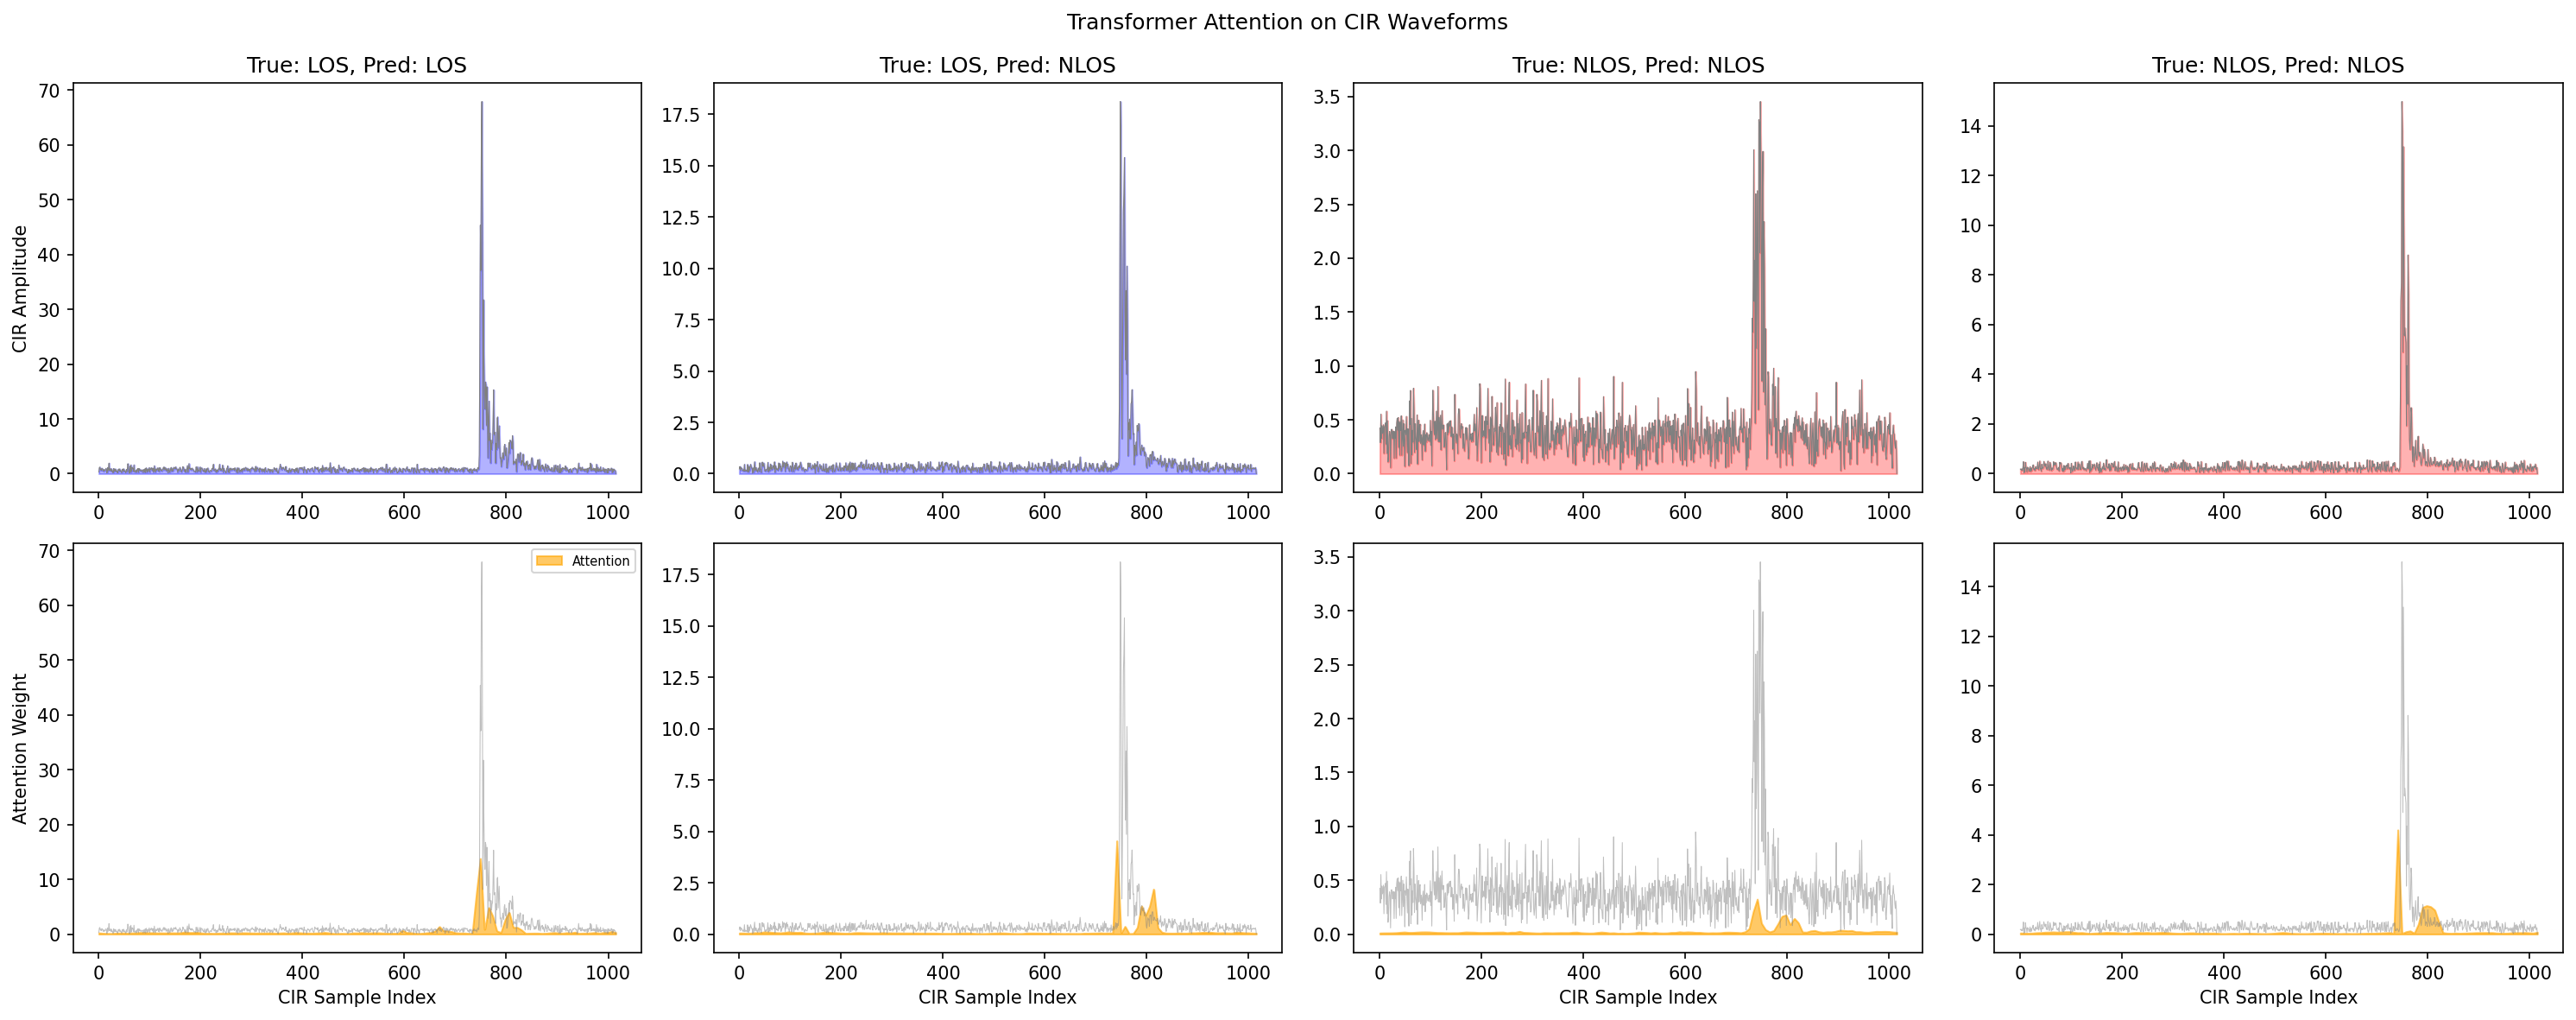
\includegraphics[width=\columnwidth]{13_attention_map.png}
\caption{Transformer attention weights overlaid on a CIR waveform. High attention concentrates near the first path and multipath components.}
\label{fig:attention}
\end{figure}

\subsection{Error Analysis}

Classification errors primarily occur in ambiguous cases where NLOS signals have strong direct-path-like characteristics or where LOS signals experience significant multipath interference. The Logistic Regression model, limited to linear decision boundaries, achieves notably lower AUC (0.9694), confirming that the LOS/NLOS boundary is inherently nonlinear.

For distance estimation, path~1 regression is more challenging ($R^2 \approx 0.64$) because the measured range includes NLOS bias errors that depend on the environment geometry rather than CIR features alone. Path~2 regression benefits from the direct geometric relationship between CIR peak positions and propagation distance.

\subsection{Model Complexity}

Table~\ref{tab:complexity} compares model complexity. The CNN-Transformer has substantially more parameters but offers the advantage of requiring no manual feature engineering.

\begin{table}[t]
\caption{Model Complexity Comparison}
\label{tab:complexity}
\centering
\begin{tabular}{@{}lcc@{}}
\toprule
\textbf{Model} & \textbf{Input Dim} & \textbf{Feature Eng.} \\
\midrule
Logistic Regression & 25 & Yes (manual) \\
Random Forest & 25 & Yes (manual) \\
Gradient Boosted Trees & 25 & Yes (manual) \\
CNN-Transformer & 1016 + 11 & No (end-to-end) \\
\bottomrule
\end{tabular}
\end{table}

%======================================================================
\section{Conclusion}

We presented a comprehensive framework for UWB LOS/NLOS classification and distance estimation using dual pipelines: a feature-engineered ML approach and an end-to-end deep learning approach. Our two-path extraction method extends binary classification to the two dominant CIR paths with physically motivated labeling rules.

Key findings include: (1) Tree-based models (RF, GBT) achieve AUC of 0.9820 using 25 hand-crafted features; (2) The novel hybrid CNN-Transformer achieves AUC of 0.9821 directly from raw CIR without feature engineering; (3) Distance estimation for the second path achieves sub-meter RMSE (0.99\,m), significantly outperforming first-path estimation; (4) Transformer attention maps provide physically interpretable visualizations of which CIR regions influence classification decisions.

\subsection{Future Work}

Several directions merit further investigation: (1) Ensemble methods combining ML and DL predictions; (2) Cross-environment generalization studies using leave-one-environment-out validation; (3) Model compression and quantization for real-time deployment on embedded UWB receivers; (4) Extension to multi-class scenarios distinguishing between different NLOS propagation mechanisms (diffraction, reflection, scattering).

\section*{Acknowledgment}

The authors thank the contributors of the UWB-LOS-NLOS-Data-Set for making the dataset publicly available.

\begin{thebibliography}{00}
\bibitem{b1} Z. Sahinoglu, S. Gezici, and I. Guvenc, ``Ultra-wideband positioning systems: theoretical limits, ranging algorithms, and protocols,'' Cambridge University Press, 2008.
\bibitem{b2} H. Wymeersch, J. Lien, and M. Z. Win, ``Cooperative localization in wireless networks,'' \textit{Proc. IEEE}, vol. 97, no. 2, pp. 427--450, Feb. 2009.
\bibitem{b3} J. Khodjaev, Y. Park, and A. S. Malik, ``Survey of NLOS identification and error mitigation problems in UWB-based positioning algorithms for dense environments,'' \textit{Ann. Telecommun.}, vol. 65, pp. 301--311, 2010.
\bibitem{b4} S. Marano, W. M. Gifford, H. Wymeersch, and M. Z. Win, ``NLOS identification and mitigation for localization based on UWB experimental data,'' \textit{IEEE J. Sel. Areas Commun.}, vol. 28, no. 7, pp. 1026--1035, Sep. 2010.
\bibitem{b5} A. Niitsoo, T. Edelhausser, E. Eberlein, N. Hadaschik, and C. Mutschler, ``A deep learning approach to position estimation from channel impulse responses,'' \textit{Sensors}, vol. 19, no. 5, p. 1064, 2019.
\bibitem{b6} A. Vaswani, N. Shazeer, N. Parmar, J. Uszkoreit, L. Jones, A. N. Gomez, L. Kaiser, and I. Polosukhin, ``Attention is all you need,'' in \textit{Proc. NeurIPS}, 2017, pp. 5998--6008.
\bibitem{b7} K. Bregar and M. Mohorcic, ``Improving indoor localization using convolutional neural networks on computationally restricted devices,'' \textit{IEEE Access}, vol. 6, pp. 17429--17441, 2018.
\bibitem{b8} T. Chen and C. Guestrin, ``XGBoost: a scalable tree boosting system,'' in \textit{Proc. ACM SIGKDD}, 2016, pp. 785--794.
\bibitem{b9} L. Breiman, ``Random forests,'' \textit{Machine Learning}, vol. 45, no. 1, pp. 5--32, 2001.
\bibitem{b10} J. Devlin, M.-W. Chang, K. Lee, and K. Toutanova, ``BERT: pre-training of deep bidirectional transformers for language understanding,'' in \textit{Proc. NAACL-HLT}, 2019, pp. 4171--4186.
\end{thebibliography}

\end{document}
